\section*{Aufgabe 27}
\label{sec:Aufgabe4}

\subsection*{a)}
Mit den Daten aus \textit{aufg\char`_a.csv} wird zum Polynom
\begin{equation}
p(x)=ax^6+bx^5+cx^4+dx^3+ex^2+fx+g\label{eq:p}
\end{equation}
wird die Designmatrix 
\[
A \text{mit} A_\text{i,j}=f_\text{i}(x_\text{j})
\]
aufgestellt. Dabei sind $f_\text{i}(x)=x^i$ mit $i=0,1,2,3,4,5,6$.
Die Einträge des Schätzvektors
\[
\vec{â}=(A^TA)^{-1}A^T\vec{y},
\]
die im Python-Script in den Zeilen 69-72 berechnet werden, sind die Koeffizienten
\begin{align*}
a &= -1,96288194\cdot 10^{-4}\\
b &= 4,78568044\cdot 10^{-3}\\
c &= -4,52007747\cdot 10^{-2}\\
d &= 2,10566519\cdot 10^{-1}\\
e &= -5,13748208\cdot 10^{-1}\\
f &= 6,09609032\cdot 10^{-1}\\
g &= -6,74453241\cdot 10^{-2}\\
\end{align*}
Der im Python-Script in den Zeilen 74-84 erzeugte Fit des Polynoms mit diesen Koeffizienten ist in Abbildung\ref{fig:polyfit} zu sehen
\begin{figure}
\centering
\includegraphics[width=\textwidth]{build/polyfit.pdf}
\caption{Fit nach der Methode der kleinsten Quadrate.}
\label{fig:polyfit}
\end{figure}

\subsection*{b)}
Die Rechnung aus Aufgabe a) wird mit Regularisierung über die 2. Ableitung und verschiedenen Regularisierungsstärken $\lambda$ wiederholt.
Die im Python-Script in den Zeilen 87-121 erzeugten Werte für die Koeffizienten sind in Abbildung \ref{fig:koeff} und die zugehörigen fits in Abbildung \ref{fig:lambdas} zu sehen.
\begin{figure}
\centering
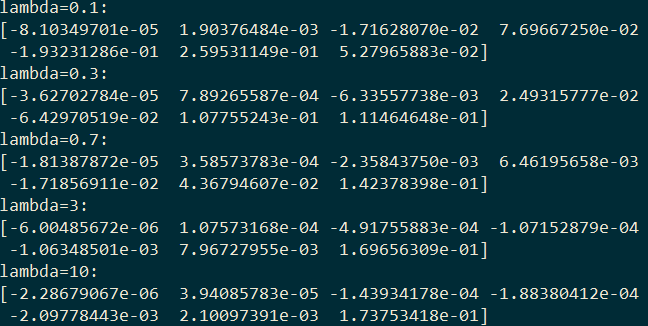
\includegraphics[width=\textwidth]{content/images/koeff.png}
\caption{Koeffizienten für verschiedene Regularisierungsstärken.}
\label{fig:koeff}
\includegraphics[width=\textwidth]{build/lambdas.pdf}
\caption{Fits für verschiedene Regularisierungsstärken.}
\label{fig:lambdas}
\end{figure}
\subsection*{c)}
Der Datensatz aus \textit{aufg\char`_c.csv} wird mithilfe von gewichteten Quadraten durch \eqref{eq:p}
gefittet. Die bestimmten Koeffizienten sind in Abbildung \ref{fig:koeff2} und der Fit in ABbildung \ref{fig:wsq} zu sehen,
Es zeigt sich deutlich, dass dieser Fit am besten zu den Daten passt.
\begin{figure}
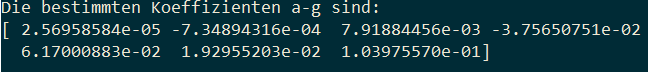
\includegraphics[width=\textwidth]{content/images/koeff2.png}
\caption{Bestimmte Koeffizienten.}
\label{fig:koeff2}
\includegraphics[width=\textwidth]{build/WSquared.pdf}
\caption{Fit mittels Methode der gewichteten Quadrate}
\label{fig:wsq}
\end{figure}
%☺◘